\newpage
\null
\vspace{0.15cm}

\begin{center}
    \Huge{\textbf{\underline{Introduction}}}
\end{center}

\setcounter{section}{0}

\vspace{0.35cm}

\section{Overview}
\begin{prettyBox}{Overview}{myblue}
We present a problem to the agent by specifying the initial situation and defining a goal. The agent then makes a series of decisions to achieve the given goal. The approaches to problem-solving can be categorized as follows: 
\begin{itemize}
    \item \textbf{Search}: Does not rely on prior experience. 
        \begin{itemize}
            \item \textbf{Uninformed Search}: Conducted without any prior information (blind search).
            \item \textbf{Informed Search}: Utilizes available information to guide the search.
        \end{itemize}
    \item \textbf{Knowledge-Based Approaches}: Relies on prior experience. 
        \begin{itemize}
            \item \textbf{Memory-Based}: Uses a database of problems and their corresponding solutions.
            \item \textbf{Rule-Based}: Converts experience into rules with human intervention.
        \end{itemize}
    \end{itemize}
\end{prettyBox}

\vspace{0.35cm}

\begin{center}
    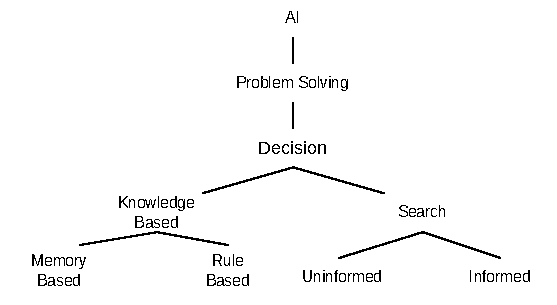
\includegraphics[height=0.4\textheight]{Chapters/Diagram/overview.drawio.pdf}
\end{center}




